
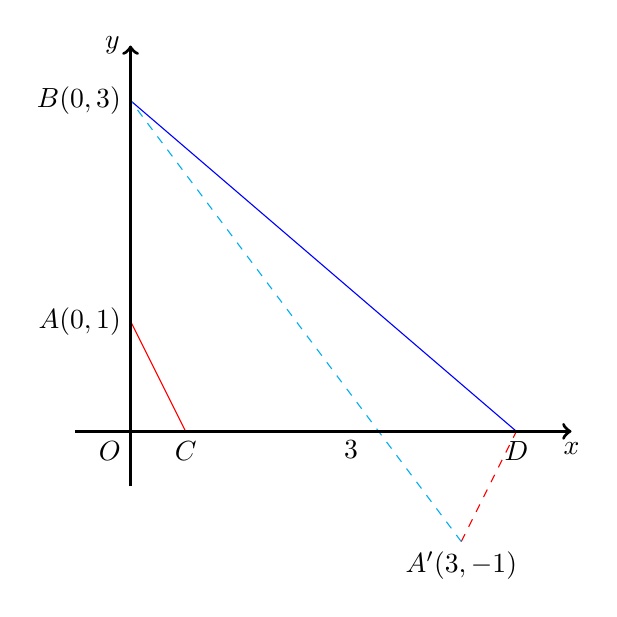
\begin{tikzpicture}[scale=1.4]
  \coordinate[label=below left:$O$] (O) at (0,0);
  \coordinate[label=left:{$A(0,1)$}] (A) at (0,1);
  \coordinate[label=left:{$B(0,3)$}] (B) at (0,3);
  \coordinate[label=below:$C$] (C) at (.5,0);
  \coordinate[label=below:$D$] (D) at (3.5,0);
  \coordinate[label=below:{$A'(3,-1)$}] (A') at (3,-1);
  \draw (C) -- node[below] {$3$} (D);
  \draw[red] (A) -- (C);
  \draw[blue] (B) -- (D);
  \draw[dashed, red] (A') -- (D);
  \draw[dashed, cyan] (A') -- (B);
  \draw[very thick, ->] (-.5,0) -- (4,0) node[below] {$x$};
  \draw[very thick, ->] (0,-.5) -- (0,3.5) node[left] {$y$};
\end{tikzpicture}
